% Histórico da kdtree:
%  - primeira proposta.
%  - Objetivo. Eficientcia
%  - Teste de colisão, pertinencia e amplitude
% Utilizacao:
The \kdtree{} is a type of binary search tree for indexing multidimensional
data with simple construction and low space usage.
Despite its simplicity it efficiently supports operations like nearest
neighbour search and range search~\cite{bentley1975}.
For those reasons \kdtree{} is widely used on
spacial geometry algorithms~\cite{preparata2012computational, guttman1984r},
clustering~\cite{kanungo2002efficient, indyk1998approximate}
and graphic rendering algorithms~\cite{owens2007survey}.

Like a standard binary search tree, the \kdtree{} subdivides data at each
recursive level of the tree.
Unlike a standard binary tree, that users only one key for all levels of the tree,
the \kdtree{} uses $k$ keys and cycles through these keys for successive levels
of the tree.

% Vantagens sobre outras estruturas (quad-tree, etc):
%  - menor sensibilidade a distribuicao tendensiosa.
% Its advantages.

Concerning it's efficiency, it is important to consider the number of dimensions
\kdtree{} is indexing.
As a general rule, a \kdtree{} is suitable for efficiently indexing of $n$ elements
if $n$ is much greater than $2^k$.
Otherwise, when \kdtree{} are used with high-dimensional data, most of the elements
in the tree will be evaluated and the efficiency is no better than exhaustive search~\cite{toth2004handbook}.

% Explicacão da indexacão das solucoes e da funcao de range.
% Indexar apenas os profits, pois nos pontos em que é necessário o range-search,
% não é necessário considerar o peso.
Indexing the solutions and range operations.

% Mencionar que esta proposta de indexacao viabiliza a aplicacão do algoritmo em problemas
% com maiores dimensões.
Tends to increase the feasibility on problems with higher dimensions.

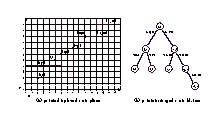
\includegraphics{src/imgs/dom-kd}
